\documentclass[twoside,11pt]{homework}
\usepackage{minted}

\coursename{Fall 2021\\COMS W4995: Parallel Functional Programming}
\teamname{Team 20}
% \reportname{Project Proposal - hGomoku}
\reportname{Project Report \\ \textbf{Gomokururu: A Go-Moku Solver}}
\studname{Kaiwen Xue, Andreas Cheng}
\studmail{\{kx2154, hc3142\}@columbia.edu}

\date{\today}

% Uncomment the next line if yofu want to use \includegraphics
\usepackage{graphicx}
\graphicspath{ {./} }


\usepackage{outlines}

\usepackage{biblatex} %Imports biblatex package
\addbibresource{reference.bib} %Import the bibliography file

\usepackage{hyperref}
\hypersetup{
    colorlinks=false,
    linkcolor=blue,
    filecolor=magenta,      
    urlcolor=cyan,
}

\begin{document}
\maketitle
% \tableofcontents
% \listoffigures

\section{Abstract}
While it is known that Go-Moku can be won by exhaustively searching the possible outcomes\cite{gomoku-solution}, such solution has a huge search space, making normal computers takes ages to perform global searching. Normally, to develop a Go-Moku AI, the search tree must be limited to a certain level. Therefore, as a computational-intensive problem, it is viable to parallel the operations in the tree search. In Gomokururu, we implemented a Go-Moku AI in haskell and applied and tested parallelism in various configurations. We found that parallelizing tree search can make minimax more efficient by tweaking various parameters of haskell's parallelism library.

\section{Introduction}
Gomoku (or Five in a Row) is a chess game where two players place black and white chess in turn on a board. The game board is formed by $N \times N$ horizontal lines. N is traditionally 15 or 19, where N=19 is an older standard that people Gomoku on a Go Board. Players should place chess on the intersection of these lines. The player assigned to the black chess plays first. The goal is to form a consecutive shape of 5 chess, which could be vertical, horizontal, or diagonal.

Minimax algorithm is based on a DFS tree search. Each tree node represents a possible state of the game. Tree leaves can be evaluated using a heuristic functions. Each layer of the tree will attempt to maximize and minimize the final outcome alternatively. Minimax is often used in game decisions where there are 1) opponents, and 2) the heuristic function can reflect the possibility of winning the game. When the tree search is sequential, alpha-beta pruning can cut the branches to prevent evaluating unnecessary game states.

% I'm not sure whether we should mention them
% There are a number of Go-Moku AIs implemented in various languages. We choose two of them and discuss how our design is better than theirs.

% \section{Goals}
% The major goal of this project is to design a Gomoku AI. AI of this type usually uses \textbf{mini-max and alpha-beta pruning}. The size of the chessboard is big (the choice space of each move), and the number of moves is also at least 20-30 (one has to have at least 5 chess on the board to win). 
% Therefore, the board states needed for the AI algorithm to work require a great amount of computation, making parallelism important. 
% Without parallelism, players will have to wait much longer than if they play with human players.

% We have found several sequential Gomoku AI implementations in various languages.
% \begin{enumerate}
%     \item https://github.com/sowakarol/gomoku-haskell. This is an AI written in sequential Haskell. Although this AI is fast (2-3 seconds response time), it is ill-designed. We ran the algorithm, and a player can win in 5 steps. Even if the player places 4 consecutive chess, the AI will not attempt to stop the expansion.
%     \item https://github.com/lukesalamone/gomoku-2049. This is an AI written in JavaScript. Although it is not ill-designed, it is not responsive. After around 10 moves, the player must wait a very long time for the computation to be done.
% \end{enumerate}

% Our goal is to do better than all of the algorithms above and create an AI that could play well with the player. That is, the player faces similar difficulty and wait a similar amount of time as if they play with a human player. We will use ThreadScope and timers to determine whether our implementation is better.

\section{Design and Implementation}
The codes listed at the end of this report are based on our favored setting, which will be discussed in  \hyperref[experiment]{Experiment Section}. Nevertheless, we have tested different settings to compare the performance of different kinds of parallelism. The full code and instructions to reproduce our results can be found at our public GitHub repository: \url{https://github.com/KevinRSX/gomokururu}.

\subsection{Data Structures}
First, to play a chess game, one will need a chess. Our implementation names it as \texttt{Piece}. It represents the state of a grid on the board, so a \texttt{Piece} can be black, white, or empty.
\begin{minted}{haskell}
data Piece = White | Black | Empty deriving (Eq)
\end{minted}

With the states of grids, we can create a chess board. The \texttt{Board} data structure contains a dimension \texttt{dim}, representing how many rows and columns it has, as well as a 2D vector that stores \texttt{dim * dim} grids. Note that we use the \texttt{Data.Vector} package to create this 2D vector. The reason is that \texttt{Vector} can ensure random access time of $O(1)$, making it much master to query.
\begin{minted}{haskell}
data Board = Board { dim :: Int
                   , getBoard :: Vector (Vector Piece) }
                   deriving (Show)
\end{minted}

All our codes are based on these two structures.

\subsection{Playing the Game}

Our implementation follows the general rules in Go-moku. Players take turn to place a piece until the board is full or a player completes a five-in-a-row. The first case is a tie and that player in the latter case is a winner. One interesting part in our implementation is our winning checking function. \textbf{We designed a way that could possibly reduce the the complexity of the function. Instead of searching five-in-a-row in the whole board, we simply search it based on the last placed piece.}

Our winning checking function takes three arguments: row, col, and board. row and col are for representing the last placed piece on the board.

With this, we can check the winning status by simply checking the "star lines" with the last placed piece as the centroid. By "star lines," we mean the horizontal, vertical, and diagonal lines that pass through the last placed piece. An ASCII representation is shown below in the code snippet.

\begin{minted}{haskell}
chkBoardWinning row col board
  | Black `elem` res && White `elem` res = error "Tie? IMPOSSIBLE!!!"
  | null res = Nothing
  | otherwise = Just $ head res
  -- length res > 1 is possible : more than 5 pieces in a row
    where res = mapMaybe whoIsWinning5 sls
          sls = getStarLines row col 5 board

whoIsWinning :: [Piece] -> Int -> Maybe Piece
whoIsWinning line cLen = helper (group line) cLen
  where
    helper :: [[Piece]] -> Int -> Maybe Piece
    helper [] cLen = Nothing
    helper (x:xs) cLen
      | length x >= cLen && head x /= Empty = Just $ head x
      | otherwise = helper xs cLen

whoIsWinning5 :: [Piece] -> Maybe Piece
whoIsWinning5 line = whoIsWinning line 5

{-
Star lines
4   4   4
 3  3  3 
  2 2 2  
   111   
432101234
   111   
  2 2 2  
 3  3  3 
4   4   4

-}
\end{minted}

\subsection{AI}
We implement this part with reference to \cite{past-project}, with improvements of the running efficiency and coding style.

\subsubsection{Minimax and Alpha-Beta Pruning}
To perform minimax, we generate a game tree of a given maximum level using the \texttt{Data.Tree} package. Note that we only include neighbors as tree nodes. Unlike in Go, which requires occupying space on the board, it is meaningless not to place chess where there is no neighbors. This approach significantly reduce the tree size.

Code wise, minimax and Alpha-Beta pruning can be done at the same time, as the latter is just cutting branchese for the former. The minimizer will call the maximizer at the next level, while the maximizer will call the minimizer at the next level. If there exists a value indicating that the rest of the branch can be discarded, the algorithm will return a value. In addition, if the heuristic calculated at a node exceeds the cutoff point, meaning that the game will win or lose if the player choose that step, the rest of the tree search will also be discarded, as this is necessarily the best move. We only include the maximizer here, and the minimizer will be similar, except that it will call the maximizer to get new beta value and choose the minimum max value. The code listed at the end of the report does not perform alpha-beta pruning, as we discard alpha-beta pruning to reach better results for parallelism.

\begin{minted}{haskell}
maxAlpha :: Piece -> Int -> Int -> Int -> Tree Board -> Int
maxAlpha _ _ alpha _ (Node _ []) = alpha
maxAlpha piece lvl alpha beta (Node b (x:xs))
  | lvl == 0 = curScore
  | canFinish curScore = curScore
  | newAlpha >= beta = beta
  | otherwise = maxAlpha piece lvl newAlpha beta (Node b xs)
  where
    curScore = computeScore b piece
    canFinish score = score > cutoffScore
    newAlpha = max alpha $ minBeta piece (lvl - 1) alpha beta x
\end{minted}


\subsubsection{AI Entry Point}
The entry point of the AI is \texttt{getNextPos}, which takes a \texttt{Board} and the current color of the chess and calls minimax to select the position for the next move.

\subsubsection{Heuristic}
There are many heuristic functions for Go-Moku with varying performance. In this project, we designed our own. First, we will find consecutive pieces -- the more consecutive pieces there are, the higher chance the player will win. However, consecutive pieces blocked by the opponent will be useless. We therefore award no score if both ends are blocked, a low score if one end is block, and a high score if both ends are empty. This can be easily achieved using pattern matching:
\begin{minted}{haskell}
> [a, b, c, d, e] == [Empty, piece, piece, piece, Empty]
    = 100 + lineScore3 piece (b:c:d:e:xs)
> [a, b, c, d, e] == [reversePiece piece, piece, piece, piece, Empty]
    || [a, b, c, d, e] == [Empty, piece, piece, piece, reversePiece piece]
    = 50 + lineScore3 piece (b:c:d:e:xs)
> otherwise = lineScore3 piece (b:c:d:e:xs)
\end{minted}

\subsection{Parallelism}
The tree search nature of the minimax nature makes it possible and suitable to use haskell's parallel techniques. In particular, we implement parallelism at two places: minimax tree search and heuristic calculation

\subsubsection{Parallelizing Minimax Tree Search}
Haskell's \texttt{Data.Tree} package represents the children of a tree in a list, i.e., \texttt{[Tree a]}. Minimax's aim is to calculate the maximum value of the score of the first node layer. Therefore, \texttt{parMap} comes in handy, as we are supposed to use \texttt{Data.List.map} to perform sequential computation.
\begin{minted}{haskell}
minmax = parMap rdeepseq (minBeta piece searchLevel) children
\end{minted}

However, this only parallelize the first level of computation. All the subtrees are not parallelized. Indeed, the challenge here is posed by the data dependency of alpha-beta pruning. Alpha-beta pruning assumes a completely sequential operation, as it will always compare the value calculated at one point to the maximum or minimum value in the previous computation in order to decide if one branch can be cut. We therefore decide not to use alpha-beta pruning in our parallel implementation. Nevertheless, not using alpha-beta pruning does not mean we do not benefit from pruning. We will calculate the score for the node beforehand continuing to the next level, and if the score is high enough to ensure a winning condition, the AI will directly choose this node.

In addition, we note that it is also important to control the degree of parallelism. If that degree is too high, the overhead due to creating sparks will exceed the reduced time due to parallelism, making parallelism meaningless. To do this, we only parallelize the first few levels of minimax searching, but keep the rest sequential.

\subsubsection{Parallelizing the Computation of Heuristic}
The computation of heuristic is also expensive, as we need to apply different functions detecting different numbers of consecutive pieces to the board. In addition, lines to be extracted from the board can be horizontal, vertical, and diagonal. To coordinate this, we use a map-reduce-like method. First, we "map" the board by extracting lines of different directions, and assign workers to calculate the partial heuristic score, and then "reduce" the calculated score by each worker to a final score. The \texttt{Eval} monad comes in handy:

\begin{minted}{haskell}
runEval $ do
  ls2 <- rpar (force (map (lineScore2 piece) pieces))
  ls3 <- rpar (force (map (lineScore3 piece) pieces))
  ls4 <- rpar (force (map (lineScore4 piece) pieces))
  ls5 <- rpar (force (map (lineScore5 piece) pieces))
  rseq ls2
  rseq ls3
  rseq ls4
  rseq ls5
  return (sum ls2 + sum ls3 + sum ls4 + sum ls5)
\end{minted}{haskell}

Note that the \texttt{map} functions can also be parallized. We will discuss the performance of different configurations in the following section.

\subsection{Tweakable Parameters}
In order to ensure that both our sequential and parallel algorithm balance efficiency and the smartness of the AI, we parameterize some constants so that we can test for their most appropriate values. First is the number of layers to be searched by minimax, second is the number of layers to be evaluated sequentially to prevent overheads, and the third is the cutoff score for minimax to stop searching for another level.

\begin{minted}{haskell}
searchLevel :: Int
searchLevel = 2

sequentialLevel :: Int
sequentialLevel = 0 -- level to be evaluated sequentially, must be
                    -- less than or equal to searchLevel

cutoffScore :: Int
cutoffScore = 1000
\end{minted}{haskell}


\section{Evaluation}
Our benchmarks include the following:
\begin{enumerate}
    \item Running time
    \item Spark statistics
    \item ThreadScope graphs
    \item Subjective observation of whether the AI is smart
\end{enumerate}

We use the following 5-tuple to represent our setup: \texttt{(mode, coreNum, searchLevel, sequentialLevel, parMapHeuristic)}. \texttt{mode} can be either \texttt{seq}, \texttt{par}, \texttt{parAB}, meaning we run the sequential alpha-beta pruning version, the complete parallel version, or the parallel version that only parallelize the first tree level and use alpha-beta pruning to handle the rest. \texttt{coreNum} indicates with how many cores we run the experiment. \texttt{searchLevel} and \texttt{sequentialLevel} are tweakable parameters discussed in the previous section. Note that with \texttt{seq} or \texttt{parAB}, we do not use \texttt{sequentialLevel}. \texttt{parMapHeuristic} is a boolean, meaning whether nor not we will use \texttt{parMap} to parallel inside each worker when computing heuristic. We run each setup for 3 times and calculate the average running time. For the other metrics, we will describe the result from one of the tests.

Experiments are run on a 2018 MacBook Pro, with 2.7 GHz Quad-Core Intel Core i7 processor. We expect the results to be much faster on desktop machines.

Note that since different setup will result in different number of steps for two AIs finish the game. The run time is the program run time divided by the number of steps in a game.

\subsection{Number of Cores}
To ensure fairness of different testings, we restrict the number of steps to 20. In this experiment, we only consider the difference among different number of cores in a completely parallel setting.

Table \ref{diff-cores} shows the comparison of run time and spark statistics for \texttt{(par, N1, 3, 1, False)}, \texttt{(par, N2, 3, 1, False)}, and \texttt{(par, N4, 3, 1, False)}:

\begin{table}[h!]
\centering
\begin{tabular}{||c c c c c c||} 
 \hline
 Core & Time per step & Total & Converted & GC'd & Fizzled \\ [0.5ex] 
 \hline\hline
 1 & 4.04 & 1238280 & 0 & 913176 & 325104 \\ 
 2 & 2.19 & 1238340 & 1343 & 904299 & 332698 \\
 4 & 1.36 & 1238724 & 14765 & 865567 & 358392 \\ [1ex] 
 \hline
\end{tabular}
\caption{Different cores}
\label{diff-cores}
\end{table}

It can be seen that multi-core leads to a significant amount of performance increase in our implementation. The quad-core system can gain a 2.97$\times$ performance increase, and the double-core system can gain a 1.61$\times$ performance increase. In addition, the spark conversion rate is also higher in multi-core setting. Doubling the number of cores will increase the conversion rate in a magnitude.

ThreadScope's output also shows that by using \textt{parMap}, the workload is balanced evenly, and the garbage collection does not take majority of time.

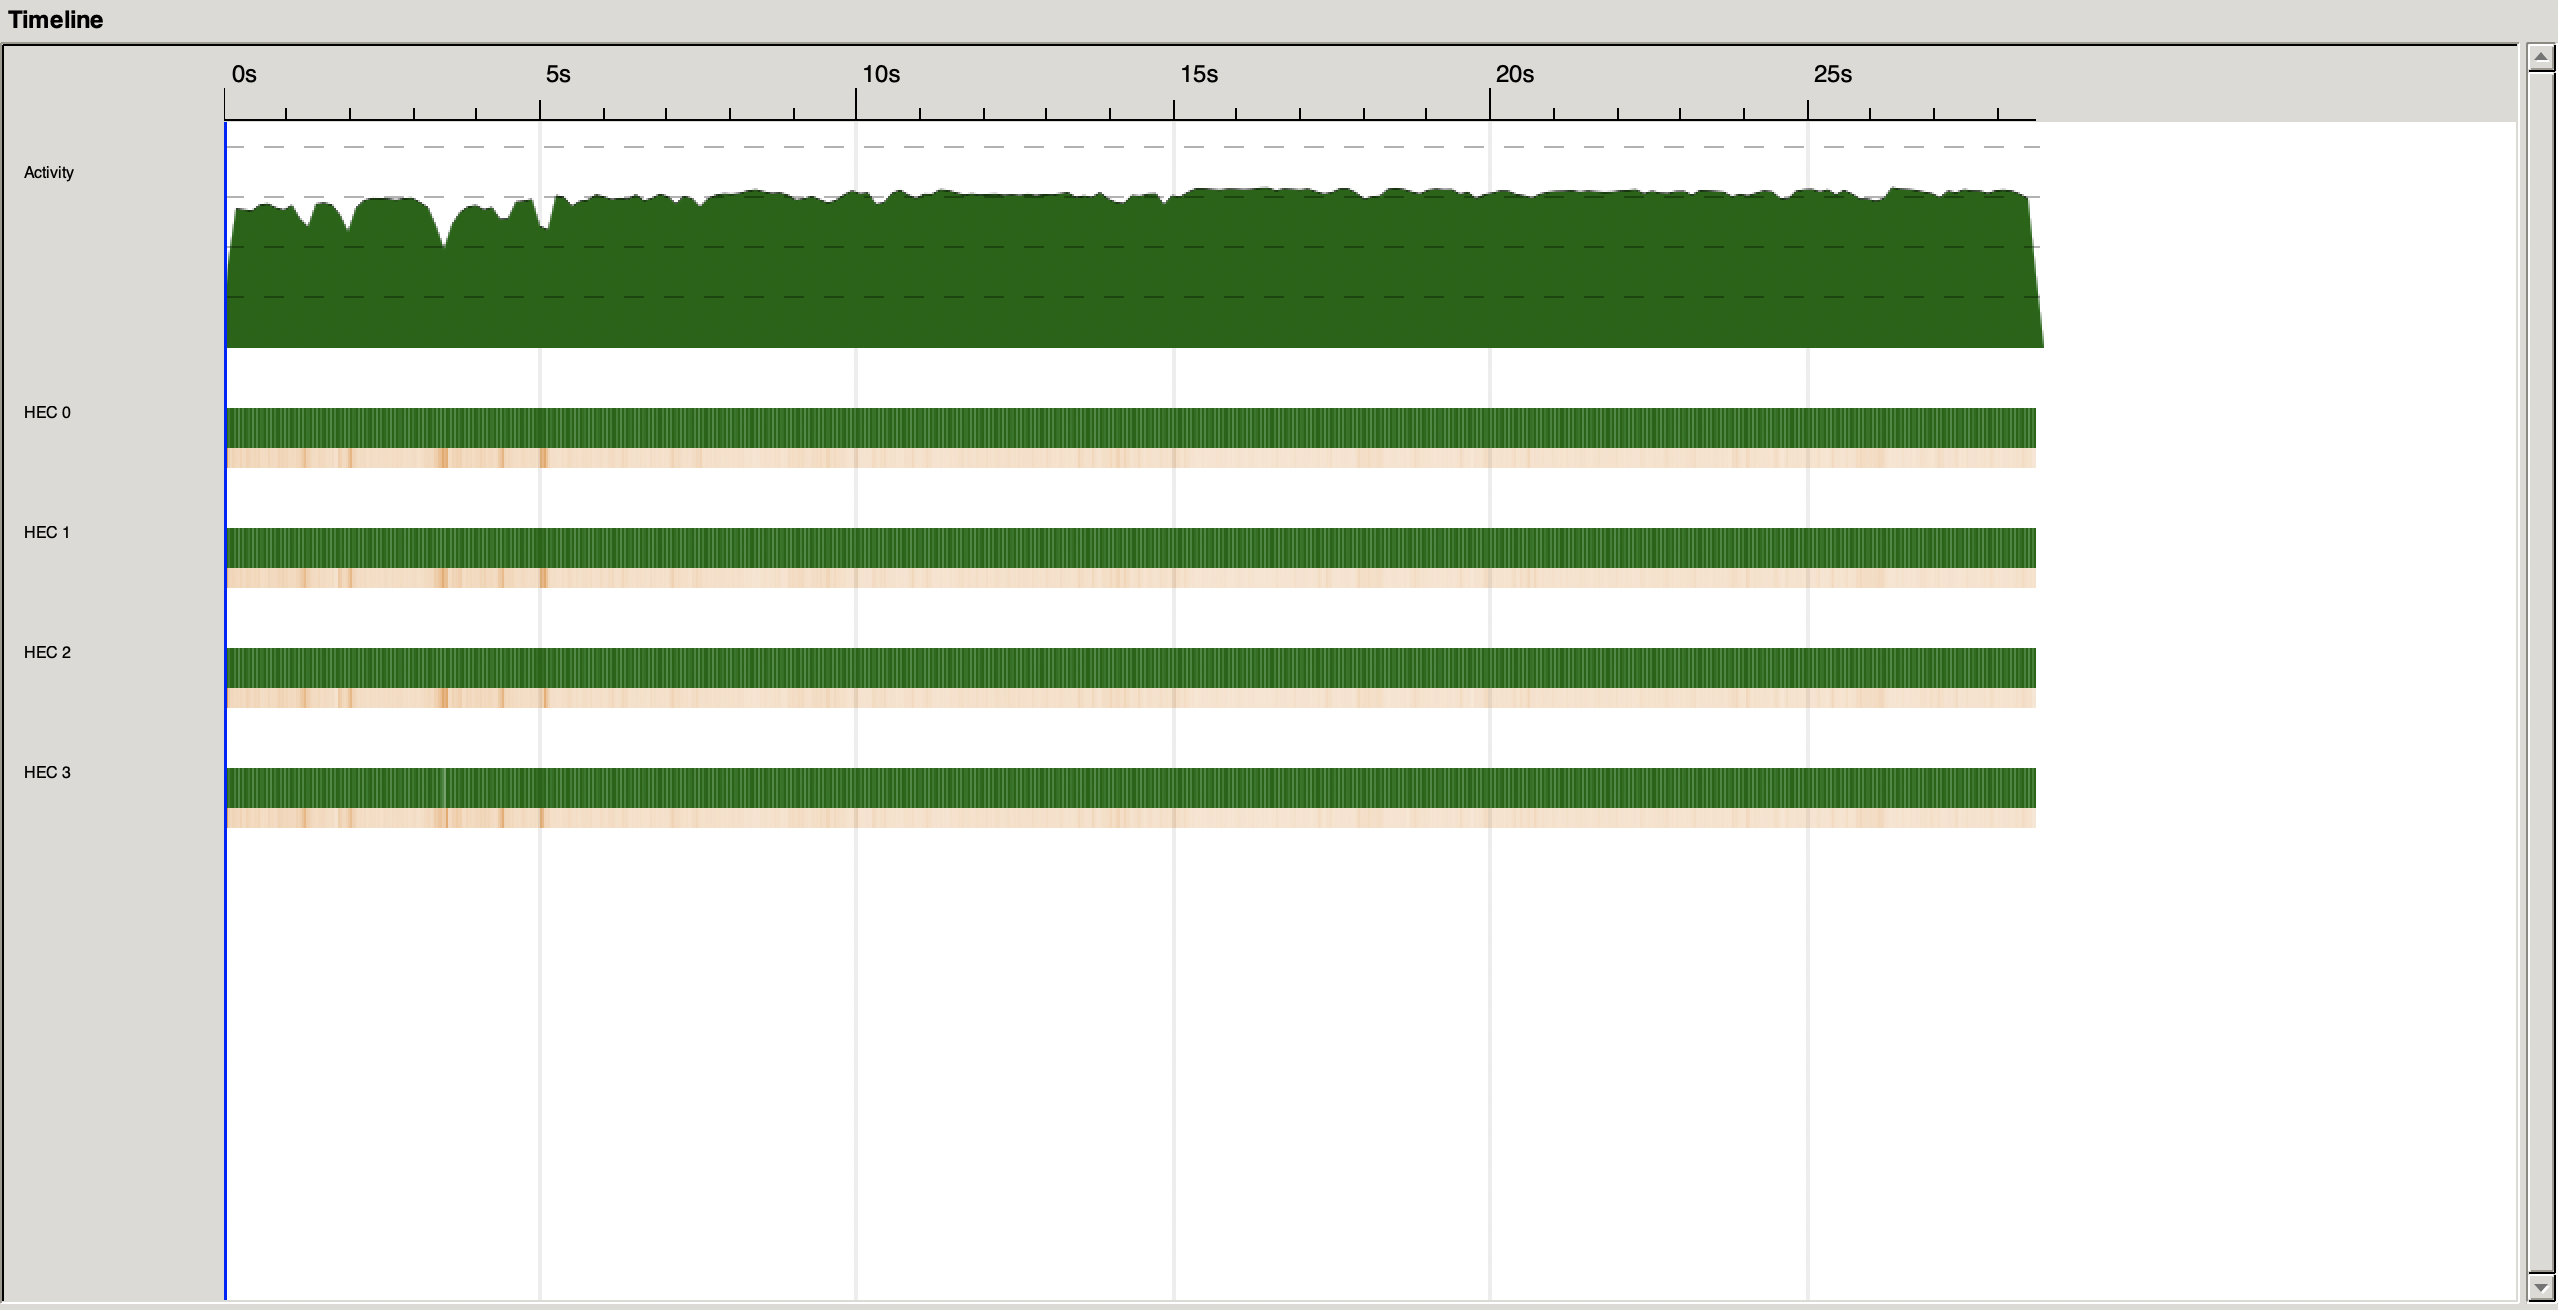
\includegraphics[scale=0.3]{par_n4_2_1_false.png}

\subsection{Parallelizing Worker Threads of Heuristic Computation}
As mentioned in the above section, the "reduce" part of the heuristic computation can be further parallelized so that each worker thread will call \texttt{parMap}. Table \ref{parMap-heuristic-workers} shows its result against the previous one in four cores.

\begin{table}[h!]
\centering
\begin{tabular}{||c c c c c c||} 
 \hline
 Setting & Time per step & Total & Converted & GC'd & Fizzled \\ [0.5ex] 
 \hline\hline
 \texttt{(par, N4, 3, 1, False)} & 1.36 & 1238724 & 14765 & 865567 & 358392 \\
 \texttt{(par, N4, 3, 1, True)} & 1.44 & 109536668 & 69214 & 107421589 & 204586 \\ [1ex] 
 \hline
\end{tabular}
\caption{parMap the heuristic worker threads}
\label{parMap-heuristic-workers}
\end{table}

As shown in the table, the time per step after parallelize the worker threads even increases slightly, showing that the overhead surpluses the benefit of parallelism. In addition, the number of sparks in this case is 100$\times$ the original sequential case. Therefore, this design is undesirable and the worker threads should be sequentially evaluated.

\subsection{Depth of Search Level}
The knowledge of game is key to winning. Balancing efficiency with knowledge is therefore important. As have shown above, we have picked \texttt{searchLevel=3}. Based on our experience playing Go-Moku, we categorize the subjective smartness of the AI in "Good", "Reasonable", and "Bad", where "Good" means the AI is able to make most moves that experienced human players would agree, "Reasonable" means the AI's move might not be consistent with experienced human players' choice but reflect some degree of smartness, and "Bad" means the AI's move is completely unreasonable. We expect our AI to be at least "Good", since the reason to build an AI is to let it compete with human.

\begin{table}[h!]
\centering
\begin{tabular}{||c c c||} 
 \hline
 Setting & Time per step & Smartness \\ [0.5ex] 
 \hline\hline
 \texttt{(par, N4, 4, 1, False)} & N.A. & Good \\
 \texttt{(par, N4, 3, 1, False)} & 1.36 & Good \\ [1ex]
 \texttt{(par, N4, 2, 1, False)} & 0.14 & Reasonable \\
 \texttt{(par, N4, 1, 1, False)} & 0.01* & Bad \\
 \hline
\end{tabular}
\\ \\ * One player wins before finishing 20 steps
\caption{parMap the heuristic worker threads}
\label{parMap-heuristic-workers}
\end{table}

If we use 4 levels, a step cannot be performed within a reasonable amount of time starting from step 10. With 1 or 2 levels, while the computation speed is extremely fast, the smartness is just "Reasonable." The time per step for 3 levels is within the patience of human. This justifies our choice to use 3 levels as our best setting.

\subsection{Partial Parallelism of Tree Search}
As noted above, parallelizing a part of the tree, while sequentially evaluating the rest, might reduce the performance decay caused by overhead of useless spark creation. In this part, we use a range of different settings by modifying $sequentialLevel$ to evaluate different choices of partial parallelism.

\begin{table}[h!]
\centering
\begin{tabular}{||c c c c c||} 
 \hline
 Setting & Steps & Time/Step & Total & Converted \\ [0.5ex] 
 \hline\hline
 \texttt{(par, N4, 4, 2, False)} & 10 & 6.08 & 3160731 & 11690 \\ 
 \texttt{(par, N4, 4, 3, False)} & 10 & 8.74 & 2808749 & 227567 \\ 
 \texttt{(par, N4, 3, 0, False)} & 20 & 1.37 & 1379813 & 11414 \\
 \texttt{(par, N4, 3, 1, False)} & 20 & 1.36 & 1238724 & 14765 \\
 \texttt{(par, N4, 3, 2, False)} & 20 & 1.57 & 1226022 & 35394 \\ [1ex] 
 \hline
\end{tabular}
\caption{parMap the heuristic worker threads}
\label{parMap-heuristic-workers}
\end{table}

Note that when \texttt{searchLevel == sequentialLevel}, all levels will be evaluated sequentially and the minimax will be completely sequential. Since we only care about \texttt{mode=par} here, we do not test such case. Instead, we evaluate it in the following section. When \texttt{searchLevel=3}, we can see that both the efficiency and cost of sparks do not differ much. However, we also compute the performance of \texttt{searchLevel=4}. We found that evaluating only 1 level in parallel will hurt the performance. Therefore, we conclude that for searching that are in 3 or 4 levels, it is reasonable to use as fewer sequential searching levels as possible, since the overhead will not reversely effect the performance.

\subsection{Parallel vs Sequential}
An important design choice we made in our parallel implementation is that we discard alpha-beta pruning. Therefore, it is important to test if this choice improvese the performance.

\begin{table}[h!]
\centering
\begin{tabular}{||c c c||} 
 \hline
 Setting & Time/Step & Smartness \\ [0.5ex] 
 \hline\hline
 \texttt{(par, N4, 3, 1, False)} & 1.36 & Good \\
 \texttt{(seqAB, N4, 3, 3, False)} & 1.07 & Reasonable \\
 \texttt{(seqAB, N1, 3, 3, False)} & 0.89 & Reasonable \\
 \texttt{(seq, N4, 3, 3, False)} & 5.10 & Good \\ [1ex] 
 \hline
\end{tabular}
\caption{Parallel vs Sequential}
\label{parallel-vs-sequential}
\end{table}

The running time per step for a sequential AI without alpha-beta pruning is the slowest. What is interesting is the parallel solution's comparison with \texttt{seqAB}. The running time is similar and even slower for parallel solution, while the smartness is better. This is due to the fact that alpha-beta pruning does not gain all the information of the tree of a certain level. In addition, we can see that alpha-beta pruning does not gain any benefit from multicore systems. If we have more than 4 cores, the performance for the parallel solution will potentially be better than the alpha-beta pruning solution.

\section{Conclusion and Future Work} \label{experiment}
Based on the experiment we have performed, we have discovered the most favorable setting for Gomokururu: \texttt{(par, N4, 3, 1, False)}. This setting balances performance, smartness of AI, and resource utilization.

However, due to time constraint, one possible improvement is not realized in this project. We can combine alpha-beta pruning with the parallel implementation by implementing the sequential part in alpha-beta pruning. This requires using two sets of minimax functions and the sequential and parallel implementation has to call each other. As all the code are open-sourced on GitHub, we welcome contributors collaborate us to make this improvement.

\section{Contribution from Team Members}
\begin{itemize}
  \item Andreas Cheng: Data structures, game board, UI, test suite, winning check, heuristic, neighbor finding
  \item Kaiwen Xue: Data structures, game board, heuristic, tree building, minimax, parallelism
\end{itemize}
\newpage

\section{Code Listing}
\subsection{Our Core Code}
\begin{minted}{haskell}
boardDiff :: Board -> Board -> (Int, Int)
boardDiff oldBoard newBoard = (drow, dcol) 
  where (drow, dcol) = quotRem diffPos (dim newBoard)
        diffPos = getDiff oldBoard1d newBoard1d 0
        getDiff [] [] _ = error "Invalid parameters"
        getDiff (x:xs) (y:ys) ind | x /= y = ind
                                  | x == y = getDiff xs ys (ind + 1)
        oldBoard1d = (V.toList . V.concat . V.toList) (getBoard oldBoard)
        newBoard1d = (V.toList . V.concat . V.toList) (getBoard newBoard)
\end{minted}

\printbibliography %Prints bibliography

\end{document} 